\documentclass[11pt,a4paper]{book}

\usepackage{Appunti}

\definecolor{groovyblue}{HTML}{0000A0}
\definecolor{groovygreen}{HTML}{008000}
\definecolor{darkgray}{rgb}{.4,.4,.4}
 
\lstdefinelanguage{Groovy}[]{Java}{
  keywordstyle=\color{groovyblue}\bfseries,
  stringstyle=\color{groovygreen}\ttfamily,
  keywords=[3]{each, findAll, groupBy, collect, inject, eachWithIndex},
  morekeywords={def, as, in, use},
  moredelim=[is][\textcolor{darkgray}]{\%\%}{\%\%},
  moredelim=[il][\textcolor{darkgray}]{§§}
}

\begin{document}
\title{The Complete Apache Groovy Developer Course}
\author{Jacopo De Angelis}
\maketitle

\pagebreak
\tableofcontents
\pagebreak

\chapter{Introduzione}
\section{groovysh}
Groovysh è un'applicazione da linea di comando fornita tramite l'SDK. Per accedervi basta scrivere nel prompt "groovysh" e si attiverà la shell.

Essendo un linguaggio di scripting è possibile scrivere semplici comandi da fare valutare (e.g. 1+1, println "Hello, World!").

\begin{lstlisting}[language = groovy]
groovy:000> 1+1
===> 2

groovy:000> println "Hello"
Hello
===> null
\end{lstlisting}

Groovy riconosce anche quando una linea di comando non è terminata, attendendo la valutazione e segnalandolo tramite il numero a inizio linea.
\begin{lstlisting}[language = groovy]
groovy:000> class Person {
groovy:001> def sayHello(){
groovy:002> println "Hello"
groovy:003> }
groovy:004> }
===> true

groovy:000> person = new Person()
===> Person@2dbfcf7

groovy:000> person.sayHello()
Hello
===> null
\end{lstlisting}

\section{groovyc}
É il corrispettivo di javac, lo script viene tradotto in Java bytecode.
\begin{lstlisting}[language = groovy]
groovyc -help                                                                                  
Usage: groovyc [options] <source-files>
      [<source-files>...]    The groovy source files to compile, or @-files
                               containing a list of source files to compile
      -cp, -classpath, --classpath=<path>
                             Specify where to find the class files - must be
                               first argument
      -sourcepath, --sourcepath=<path>
                             Specify where to find the source files
      --temp=<temp>          Specify temporary directory
      --encoding=<encoding>  Specify the encoding of the user class files
  -d=<dir>                   Specify where to place generated class files
  -e, --exception            Print stack trace on error
      -pa, --parameters      Generate metadata for reflection on method
                               parameter names (jdk8+ only)
      -pr, --enable-preview  Enable preview Java features (JEP 12) (jdk12+
                               only) - must be after classpath but before other
                               arguments
  -j, --jointCompilation     Attach javac compiler to compile .java files
  -b, --basescript=<class>   Base class name for scripts (must derive from
                               Script)
  -J=<property=value>        Name-value pairs to pass to javac
  -F=<flag>                  Passed to javac for joint compilation
      --indy                 Enables compilation using invokedynamic
      --configscript=<script>
                             A script for tweaking the configuration options
  -h, --help                 Show this help message and exit
  -v, --version              Print version information and exit
      --compile-static       Use CompileStatic
      --type-checked         Use TypeChecked
\end{lstlisting}

I file possono essere successivamente eseguiti tramite "groovy [file.class]".

\section{groovyConsole}
Digitare nel prompt "groovyConsole" apre la console, ovvero un ambiente di sviluppo base dove scrivere e testare i nostri script.
\begin{figure}[h!]
	\begin{center}
		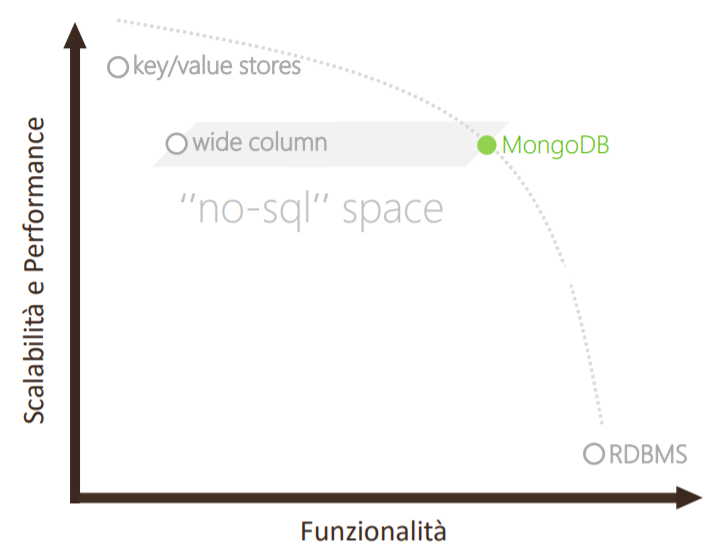
\includegraphics[scale=0.6]{img/001.png}
		\caption{Groovy console}
		\label{fig: 001}
	\end{center}
\end{figure}

\section{Alcune note per passare da Java a Groovy}
\begin{itemize}
	\item return non serve in quanto verrà automaticamente restituito l'ultimo output del metodo
	\item public non serve per gli oggetti
	\item ; non servono a meno di seperare due comandi sulla stessa linea
	\item le proprietà di un oggetto sono private di default
	\item getter e setter non servono
	\item println non necessita dei System.out. prima, è un metodo di default, le parentesi sono superflue
	\item @groovy.transform.toString() usato come annotazione sulla classe crea automaticamente la redifinizione del metodo
	\item i costruttori sono superflui in quanto posso costruire manualmente l'istanza (e.g. "new User(firstName:"nome", lastname:"cognome")"
\end{itemize}

\chapter{Le basi}
\section{Import di default}
\begin{lstlisting}[language = groovy]
import java.lang.*
import java.util.*
import java.io.*
import java.net.*
import groovy.lang.*
import groovy.util.*
import java.math.BigInteger
import java.math.BigDecimal
\end{lstlisting}
Questi import automatici riducono il boilerplate. Nel caso siano richiesti altri import è uguale a Java.

\section{Assertions}
$assert$ funziona per valutare se l'espressione successiva sia vera.

\section{Numeri}
Groovy fa un boxing automatico dei numeri nelle loro versioni oggetto (e.g. int -> Integer) 

\section{Control structure}
swtich, if e while funzionano allo stesso modo di Java eccetto che per le stringhe true vale solo se la stringa contiene un valore, la stringa vuota è false.

\subsection{for}
I for possono avere la forma iterativa
\begin{lstlisting}[language = groovy]
for(x in collection){
	...
}
\end{lstlisting}

oppure la funzione .each.

\section{Annotazioni e \href{http://docs.groovy-lang.org/next/html/gapi/groovy/transform/package-summary.html}{AST transformation}}

Prima di tutto bisogna importare il package groovy.transform.*.

Le annotazioni funzionano tramite "@codiceDell'implementazione", ad esempio:
\begin{lstlisting}[language = groovy]
import groovy.transform.Immutable

@Immutable
class Customer {
	String first, last
	int age
	Date since
	Collection favItems
}
\end{lstlisting}

In questo caso la classe sarà in sola lettura.

\section{\href{https://groovy-lang.org/operators.html}{Operatori}}
\begin{lstlisting}[language = groovy]
assert  1  + 2 == 3
assert  4  - 3 == 1
assert  3  * 5 == 15
assert  3  / 2 == 1.5
assert 10  % 3 == 1
assert  2 ** 3 == 8
assert 2++ == 3
assert 3-- == 2
\end{lstlisting}

Abbiamo anche gli operatori di assegnamento
\begin{lstlisting}[language = groovy]
def a = 4
a += 3

assert a == 7

def b = 5
b -= 3

assert b == 2

def c = 5
c *= 3

assert c == 15

def d = 10
d /= 2

assert d == 5

def e = 10
e %= 3

assert e == 1

def f = 3
f **= 2

assert f == 9
\end{lstlisting}

In groovy sono stati aggiunti === e !== che implicano identità, quindi non uguali in contenuto ma uguali in identità.
\begin{lstlisting}[language = groovy]
@EqualsAndHashCode
class Creature { String type }

def cat = new Creature(type: 'cat')
def copyCat = cat
def lion = new Creature(type: 'cat')

assert cat.equals(lion) // Java logical equality
assert cat == lion      // Groovy shorthand operator

assert cat.is(copyCat)  // Groovy identity
assert cat === copyCat  // operator shorthand
assert cat !== lion     // negated operator shorthand
\end{lstlisting}

\subsection{Elvis operator}
Novità è l'elvis operator, ovvero un'abbreviazione dell'operatore ternario
\begin{lstlisting}[language = groovy]
import groovy.transform.ToString

displayName = user.name ? user.name : 'Anonymous'   
displayName = user.name ?: 'Anonymous' 
\end{lstlisting}
Un esempio di uso
\begin{lstlisting}[language = groovy]
@ToString
class Element {
    String name
    int atomicNumber
}

def he = new Element(name: 'Helium')
he.with {
    name = name ?: 'Hydrogen'   // existing Elvis operator
    atomicNumber ?= 2           // new Elvis assignment shorthand
}
assert he.toString() == 'Element(Helium, 2)'
\end{lstlisting}

\subsection{Safe navigation}
Altro operatore utile è quello di safe navigation, il quale accede al campo se e solo se questo non è null.
\begin{lstlisting}[language = groovy]
def person = Person.find { it.id == 123 }    
def name = person?.name                      
assert name == null  
\end{lstlisting}

\section{\href{http://docs.groovy-lang.org/latest/html/documentation/grape.html}{Grave}}
É un tool di dependecy management, può essere usato in forma estesa o in forma contratta:
\begin{lstlisting}[language = groovy]
@Grab(group='org.springframework', module='spring-orm', version='3.2.5.RELEASE')
import org.springframework.jdbc.core.JdbcTemplate

@Grab('org.springframework:spring-orm:3.2.5.RELEASE')
import org.springframework.jdbc.core.JdbcTemplate
\end{lstlisting}

In questo modo non ci serve avere il jar per passare un file, verrà automaticamente risolto.

\chapter{Tipi}
var : Java = def : groovy

Solo che def è totalmente dinamico, non dobbiamo tenere lo stesos tipo di variabile, "def" implica che può contenere una qualsiasi cosa, quindi potremmo dire
\begin{lstlisting}[language = groovy]
def x = 10
x = "stringa"
\end{lstlisting}

\section{times, upto, downto, step}
times è un metodo di Integer che permette di eseguire una funzione n volte
\begin{lstlisting}[language = groovy]
20.times {
	...
}
\end{lstlisting}

upto funziona da x a y
\begin{lstlisting}[language = groovy]
1.upto(10) {
	...
}
\end{lstlisting}

downto è l'esatto contrario
\begin{lstlisting}[language = groovy]
10.downto(1) {
	...
}
\end{lstlisting}

step è come upto ma permette di stabilire l'incremento, ad esempio qua farà 0, 0.1, 0.2,...1
\begin{lstlisting}[language = groovy]
0.step(1, 0.1) {
	...
}
\end{lstlisting}

\section{Redifinizione degli operatori}
Una cosa utile è ridefinire le operazioni base in modo da potere prescrivere comportamenti specifici per nuove classi. Ad esempio, se volessimo ridefinire il + potremmo scrivere
\begin{lstlisting}[language = groovy]
[oggetto] plus([altro oggetto]){
	...
}
\end{lstlisting}

\href{https://groovy-lang.org/operators.html#Operator-Overloading}{Qua} possiamo vedere la lista delle operazioni.

\section{Stringhe}
Cosa da ricordare, se vogliamo creare una stringa multilinea bisogna rispettare un passo ulteriore, ovvero l'utilizzo del triplo apice/doppio apice:
\begin{lstlisting}[language = groovy]
def aLongMessage = '''
Questo
è
un
messaggio
multilinea
'''
\end{lstlisting}

\subsection{\$}
Le stringhe possono contenere caratteri speciali, ad esempio \, in quel caso si possono "escapare" singolarmente o in blocco, ad esempio:
\begin{lstlisting}[language = groovy]
"c:\\cartella\\interna"

// oppure

$c:\cartella\interna$
\end{lstlisting}

\section{Regex}
Funzionano come in java ma vengono dichiarate diversamente, ovvero tramite l'operatore ~.
\begin{lstlisting}[language = groovy]
def pattern = ~[regex]

def finder = text ~= pattern
def matcher = text ~== pattern
\end{lstlisting}
La differenza tra find (~=) e match (~==) è che find restituisce una lista di ritrovamenti, match restituisce un boolean che rappresenta se la stringa è generata dalla regex o no.

Un uso particolare è quello

String.replaceFirst(regex, newString) che permette di sostituire la prima istanza che viene trovata dalla regex con newString.

\chapter{Collections}
\section{\href{http://docs.groovy-lang.org/latest/html/gapi/groovy/lang/Range.html}{Range}}
I range vengono creati con un operatore particolare, ..
\begin{lstlisting}[language = groovy]
def range = 1..10
def halfRange = 1..<10
\end{lstlisting}
Questo va a definire una lista che va da 1 a 10 e una lista da 1 a 9.

Può essere usato con vari oggetti, ad esempio char e Date.

\section{\href{http://docs.groovy-lang.org/latest/html/groovy-jdk/java/util/List.html}{List} e \href{http://docs.groovy-lang.org/latest/html/groovy-jdk/java/util/Map.html}{Maps}}
Le liste funzionano in parte come array in parte come le liste in Java.

Le mappe sono come in Java ma le chiavi possono essere definite in modi differenti:
\begin{lstlisting}[language = groovy]
def varKey = key3
def map = [key1:val1, 'key2':val2, (varKey):val3]
\end{lstlisting}
key1 è convertita automaticamente in stringa, (varKey) segnala di prendere il valore della variabile.

É più conveniente leggere la documentazione.

\chapter{\href{https://groovy-lang.org/closures.html}{Closures}}
è un metodo definito come un oggetto da potere passare.

Lo definiamo in maniera simile ad una variabile.
\begin{lstlisting}[language = groovy]
def sayHello = { name ->
	println "Hello, $name!"
}

sayHello("Nome")
\end{lstlisting}

A questo punto possiamo usarlo come funzione anonima. Se vogliamo passare più di una variabile possiamo farlo. Nel seguente esempio viene passata una closure e viene usata assieme all'altra variabile num.
\begin{lstlisting}[language = groovy]
def timesTen(num, closure){
	closure(num * 10)
	
timesTen(10, { println it })
\end{lstlisting}

Notare che con it diciamo di prendere automaticamente il valore passato.

C'è anche un modo particolare per usare le closure, ovvero nel caso vengano passate come ultimo argomento, in quel caso possono essere chiamate così:
\begin{lstlisting}[language = groovy]
timesTen(10) {
	println it
}
\end{lstlisting}

Se vogliamo assicurarci che nessuna variabile possa essere passata possiamo usare l'operatore freccia vuoto
\begin{lstlisting}[language = groovy]
def noVar = { ->
     println "No var"
}
\end{lstlisting}

Se vogliamo avere un valore di default possiamo farlo. Attenzione che tutti i valori con un default devono essere messi in fondo alla lista dei valori passabili e che non possiamo decidere di usare il default del secondo e non del primo. 
\begin{lstlisting}[language = groovy]
def great = {String name, String greeting = "howdy" ->
	println "$greeting, $name"
}

great("nome")
great("Nome, "Saluto")

// Esempio di chiamata invalida
def closure = {String first, String second = "second", String third = "third" ->
	println "$first, $second, $third)
}

closure("first",,"Third") // invalida
\end{lstlisting}

Possiamo usare "var" nella definizione di un metodo. Possiamo anche dire che riceveremo una lista tramite ..
\begin{lstlisting}[language = groovy]
def concat(String.. args ->
	args.join('')
}
\end{lstlisting}

Ci sono alcune proprietà speciali di tutte le closure, ad esmepio Closure.maximumNumberOfParameters.

\section{curry}
Closure.curry ci permette di estendere una closure già esistente in modo da riempire precedentemente certi argomenti.
\begin{lstlisting}[language = groovy]
def log = { String type, Date createdOn, String msg ->
	println "$createdOn ($type) - $msg
}

log("Debug", new Date(), "This is my first statement")

def debugLog = log.curry("DEBUG")
debugLog(new Date(), "This is my second statement")

def todayLog = log.curry("DEBUG", new Date())
todayLog("This is my third statement")
\end{lstlisting}

Ci sono anche dei curry speciali, uno per partire da destra (rcurry) e uno per decidere a che indice degli argomenti riempire (ncurry(idx, arg)).

\section{Closure scope e delegate}
All'interno di una closure abbiamo tre scope:
\begin{itemize}
	\item this: corrisponde alla classe dove è definita la closure
	\item owner: corrisponde all'oggetto dove la classe è definita, la quale potrebbe essere un'altra classe o un'altra closure
	\item delegate: corrisponde ad un oggetto di terze parti dove le chiamate o le proprietà sono risolte nel caso il ricevente del messaggio non sia definito
\end{itemize}

Per capire meglio a cosa ci si riferisca serve una demo:
\begin{lstlisting}[language = groovy]
class ScopeDemo {

    def outerClosure = {
        println this.class.name // ScopeDemo
        println owner.class.name // ScopeDemo
        println delegate.class.name // ScopeDemo
        
        def nestedClosure = {
            println this.class.name // ScopeDemo
            println owner.class.name // ScopeDemo$_closure1
            println delegate.class.name // ScopeDemo$_closure1
        }
        
        nestedClosure()
    }
   
}

def demo = new ScopeDemo()
demo.outerClosure()
\end{lstlisting}

La maggiore parte delle volte owner e delegate sono uguali. Possiamo però usare il delegate in maniere partricolari, ovvero dichiarandolo:
\begin{lstlisting}[language = groovy]
def writer = {
    append "Nome"
    append " vive a Milano"
}

StringBuffer sb = new StringBuffer()
writer.delegate = sb
writer()
\end{lstlisting}

Facendo così writer non troverà metodi append definiti al suo interno, allora inizierà a cercare nell'owner e nel caso non ne trovasse allora cercherà nel delegate. Usando così delegate possiamo dire con che classe risolvere le chiamate.

\chapter{Control structure}
Le uniche due tra le condizionali che meritano di essere citate sono lo switch e in:
\begin{lstlisting}[language = groovy]
switch(num) {
    case 0 :
    case 1 :
        println num
        break
    case 1..3 :
        println "in range 1..3"
        break
    case [1, 2, 12]
        println num
        break
    case Integer:
        println "num is an Integer"
        break
    case Float:
        println "num is a float"
        break
    default:
        println "default.."
}       

def range = 18..35
def list = [1, 2, 3]

println 21 in range // true
println 4 in list // false
\end{lstlisting}

Come si può vedere si possono usare casi molto più particolari.

\section{Error Handling}
La differenza con Java è che l'eccezione nella firma del metodo è opzionale, nel caso non venga gestita all'interno del metodo allora sarà passato al chiamante.

\begin{lstlisting}[language = groovy]
// Java
public void foo() throws Exception {
	...
}

// Groovy
def foo() {
	...
}
\end{lstlisting}

\chapter{OOP}
\section{Traits}
I tratti sono dei pezzi di codici già implementati che possono essere inseriti direttamente nelle classi. Vengono aggiunti tramite implements, come se fossero interfacce; la differenza con queste è che possono mantenere uno stato.
\begin{lstlisting}[language = groovy]
trait FlyingAbility {
	private final String FLY_STRING = "I'm flying"	
	
	String fly() {
		FLY_STRING
	}
}

trait SpeakingAbility {
	String speak() {
		"I'm speaking"
	}
}
\end{lstlisting}
\begin{lstlisting}[language = groovy]
class Bird implements FlyingAbility, SpeakingAbility {
	...
}

Bird birbo = new Bird()
assert birbo.fly == "I'm flying"
assert birbo.speak == "I'm speaking"
\end{lstlisting}

\section{Serializable}
Mentre con Java le classi da serializzare sono estremamente verbose, in Groovy sono estremamente semplici grazie a ciò che viene creat OOTB da groovy. Le classi devono:
\begin{itemize}
	\item avere solo campi privati
	\item avere un costruttore senza argomenti
	\item avere getter e setter
\end{itemize}

Mentre in Java dovremmo fare tutto ciò in Groovy molto è fatto direttamente dal compilatore, quindi:
\begin{lstlisting}[language = java]
// Esempio Java

public class Person implements Serializable{
	private String firstName;
	private String lastName;
	private String email;
	
	public Person() {
	}
	
	// getter e setter, 6 metodi
}
\end{lstlisting}
\begin{lstlisting}[language = groovy]
// Esempio Groovy

class Person implements Serializable{
	String firstName, lastName, email
}
\end{lstlisting}
e fine.

\chapter{Metaprogramming}
MOP (Meta Object Protocol) è una collezione di regole di come una richiesta per un metodo è gestita dal sistema runtime di Groovy e come controllare lo strato intermedio.
\begin{figure}[h!]
	\begin{center}
		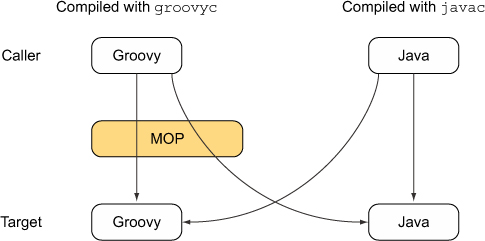
\includegraphics[scale=0.6]{img/002.jpg}
		\caption{MOP}
		\label{fig: 002}
	\end{center}
\end{figure}

\begin{figure}[h!]
	\begin{center}
		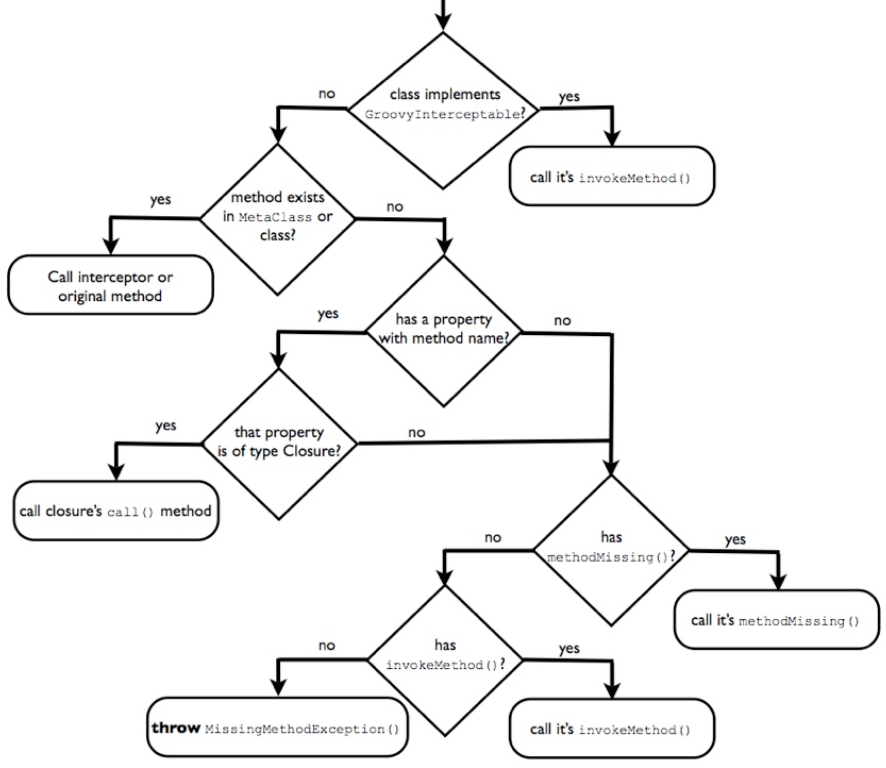
\includegraphics[scale=0.5]{img/003.png}
		\caption{Decisioni del MOP}
		\label{fig: 003}
	\end{center}
\end{figure}

Possiamo quindi personalizzare il nostro MOP con alcuni intercettori, ovvero:
\begin{itemize}
	\item invokeMethod
	\item getProperty
	\item property missing
	\item set property
	\item method missing
\end{itemize}

\section{invokeMethod}
\begin{lstlisting}[language = groovy]
class InvokeDemo {
	
	def invokeMethod(String name, Object args) {
		return "called invokeMethod $name $args"
	}
	
	def test() {
		return "method exists"
	}
}

def invokeDemo = new InvokeDemo()

assert invokeDemo.test() == "method exists"
assert invokeDemo.someMethod() == "called invokeMethod someMethod []"
\end{lstlisting}

se non avessi implementato invokeMethod il secondo assert sarebbe fallito in quanto non ci sarebbe stato alcun metodo da chiamare. In questo caso, invece, viene intercettata la chiamata ad un qualsiasi metodo e se non viene trovato quello corrispondente invokeMethod ne prende il posto, prendendo in ingresso il nome del metodo chiamato e gli argomenti passati.

\section{getProperty, setProperty, propertyMissing}
\begin{lstlisting}[language = groovy]
class PropertyDemo {
	def prop1 = "prop1"
	def prop2 = "prop2"
	def prop3 = "prop3"
}

def pd = new PropertyDemo()
assert pd.prop1 == "prop1"
assert pd.prop2 == "prop2"
assert pd.prop3 == "prop3"
\end{lstlisting}
\begin{lstlisting}[language = groovy]
class PropertyDemo {
	def prop1 = "prop1"
	def prop2 = "prop2"
	def prop3 = "prop3"
	
	def getProperty(String name) {
		println "getting property $name"
	}
}

def pd = new PropertyDemo()
assert pd.prop1 == "getting property prop1"
assert pd.prop2 == "getting property prop2"
assert pd.prop3 == "getting property prop3"
\end{lstlisting}
Anche in questo caso intercetta le chiamate ad ogni getter. Giustamente potremmo volere usare questo sistema per loggare qualcosa ma poi continuare con l'esecuzione, per quello possiamo usare le metaclass:
\begin{lstlisting}[language = groovy]
class PropertyDemo {
	def prop1 = "prop1"
	def prop2 = "prop2"
	def prop3 = "prop3"
	
	def getProperty(String name) {
		println "getting property $name"
		
		if (metaClass.hasProperty(this, name) {
			return metaClass.getProperty(this, name)
		} else {
			println "no property with name $name"
			return name
		}
	}
}
\end{lstlisting}
getProperty e setProperty lavorano sullo stesso principio. La parte dell'else però è macchinosa, è meglio gestirla tramite la propertyMissing:
\begin{lstlisting}[language = groovy]
class PropertyDemo {
	def prop1 = "prop1"
	def prop2 = "prop2"
	def prop3 = "prop3"
	
	def getProperty(String name) {
		println "getting property $name"
		return metaClass.getProperty(this, name)
	}
	
	def propertyMissing(String name) {
		println "no property with name $name"
		return name
	}
}
\end{lstlisting}

\section{methodMissing}
É invocato solo se non viene trovato un metodo con quel nome.
\begin{lstlisting}[language = groovy]
class methodMissingDevo {
	
	def methodMissing(String name, def args){
		println "Method missing with name $name"
		println "with arguments $(args)"
		if (/* condition for specific methods */) {
			throw MissingMethodException(name, args)
		}
	}
}
\end{lstlisting}

\section{Metaclass}
Le metaclassi permettono di aggiungere metodi alla classe senza aggiungerli a quella concreta, un po' come le transformation viste prima. Possiamo creare classi a runtime (classi di tipo Expando) o modificare quelle già esistenti, ad esempio:
\begin{lstlisting}[language = groovy]
Expando ex = new Expando()
e.metaClass.name = "expando"
e.metaClass.writeCode = { -> println $name }
e.writeCode()

class Developer {
	// vuota
}

Developer dev = new Developer()
dev.metaClass.name = "developer"
dev.metaClass.writeCode = { -> println $name }
dev.writeCode()
\end{lstlisting}

In questo modo stiamo aggiunendo alla classe delle proprietà senza essere limitati da quelle presenti all'interno della classe concreta.

\section{Category class}
Sono classi che racchiudono una serie di metodi applicabili in giro ma che non richiedono di essere istanziate. Il problema è che se certi metodi venissero usati senza una distinzione in una classe qualcuno potrebbe chiedersi da dove arrivino. Quindi usiamo le cateogy class. I metodi devono essere tutti statici e devono essere chiamati all'interno di un blocco use.
\begin{lstlisting}[language = groovy]
def StringCategory {
	static String shout(String str) {
		str.toUpperCase()
	}
}

use(StringCategory){
	println "Hello, world!".shout	
}

println "Hello, world!".shout() // Error
\end{lstlisting}
Per usare un esempio OOTB c'è la TimeCategory:
\begin{lstlisting}[language = groovy]
use(TimeCategory) {
	println 1.minute.from.now
	
	def someDate = new Date()
	println someDate - 3.month
}
\end{lstlisting}

\chapter{Materiali utili}
\href{https://groovy-lang.org/}{Documentazione}

\href{https://www.manning.com/books/groovy-in-action-second-edition}{Groovy in action}

\href{https://www.manning.com/books/making-java-groovy}{Making Java Groovy}

\href{https://pragprog.com/titles/vslg2/programming-groovy-2/}{Programming Groovy 2}
\end{document}